\documentclass[12pt,letterpaper]{article}
\usepackage{graphicx,textcomp}
\usepackage{natbib}
\usepackage{setspace}
\usepackage{fullpage}
\usepackage{color}
\usepackage[reqno]{amsmath}
\usepackage{amsthm}
\usepackage{fancyvrb}
\usepackage{amssymb,enumerate}
\usepackage[all]{xy}
\usepackage{endnotes}
\usepackage{lscape}
\newtheorem{com}{Comment}
\usepackage{float}
\usepackage{hyperref}
\newtheorem{lem} {Lemma}
\newtheorem{prop}{Proposition}
\newtheorem{thm}{Theorem}
\newtheorem{defn}{Definition}
\newtheorem{cor}{Corollary}
\newtheorem{obs}{Observation}
\usepackage[compact]{titlesec}
\usepackage{dcolumn}
\usepackage{tikz}
\usetikzlibrary{arrows}
\usepackage{multirow}
\usepackage{xcolor}
\newcolumntype{.}{D{.}{.}{-1}}
\newcolumntype{d}[1]{D{.}{.}{#1}}
\definecolor{light-gray}{gray}{0.65}
\usepackage{url}
\usepackage{listings}
\usepackage{color}

\definecolor{codegreen}{rgb}{0,0.6,0}
\definecolor{codegray}{rgb}{0.5,0.5,0.5}
\definecolor{codepurple}{rgb}{0.58,0,0.82}
\definecolor{backcolour}{rgb}{0.95,0.95,0.92}

\lstdefinestyle{mystyle}{
	backgroundcolor=\color{backcolour},   
	commentstyle=\color{codegreen},
	keywordstyle=\color{magenta},
	numberstyle=\tiny\color{codegray},
	stringstyle=\color{codepurple},
	basicstyle=\footnotesize,
	breakatwhitespace=false,         
	breaklines=true,                 
	captionpos=b,                    
	keepspaces=true,                 
	numbers=left,                    
	numbersep=5pt,                  
	showspaces=false,                
	showstringspaces=false,
	showtabs=false,                  
	tabsize=2
}
\lstset{style=mystyle}
\newcommand{\Sref}[1]{Section~\ref{#1}}
\newtheorem{hyp}{Hypothesis}


\title{Problem Set 1: Solution}
\date{Due: October 1, 2023}
\author{\textcolor{blue}{Student: Shekhar Kedia (23351315)}\\
	Applied Stats/Quant Methods 1}

\begin{document}
\maketitle

\section*{Instructions}
	\begin{itemize}
	\item Please show your work! You may lose points by simply writing in the answer. If the problem requires you to execute commands in \texttt{R}, please include the code you used to get your answers. Please also include the \texttt{.R} file that contains your code. If you are not sure if work needs to be shown for a particular problem, please ask.
	\item Your homework should be submitted electronically on GitHub.
	\item This problem set is due before 23:59 on Sunday October 1, 2023. No late assignments will be accepted.
	\item Total available points for this homework is 80.
	\end{itemize}	
\vspace{0.5cm}

\textcolor{blue}{
\section*{Notes:}
\begin{itemize}
	\item Please note, the responses are nested right after each problem in blue colour.\\ For instance-\\ \texttt{For problem 1.1}, the responses are mentioned right after the question for \texttt{1.1}.
	\item The format for response is in the following manner:
	\subitem - Steps to be followed
	\subitem - The \texttt{R} script
	\subitem - Interpretation of result
	\item The example \texttt{.R} file and \texttt{.tex} file that was provided, is modified to develop this document.
	\item My knowledge of library packages in both \texttt{R} and \texttt{LaTeX} is limited and so, I might have attached packages which are either redundant or unnecessary in doing this assignment.
\end{itemize}	
\vspace{0.5cm}
}	

\pagebreak
\section*{Question 1 (40 points): Education}
A school counselor was curious about the average of IQ of the students in her school and took a random sample of 25 students' IQ scores. The following is the data set:\\

\lstinputlisting[language=R, firstline=42, lastline=43]{PS01_answers_SK.R}  

\begin{enumerate}
	\item Find a 90\% confidence interval for the average student IQ in the school.

\vspace{0.25cm}

\textcolor{blue}{
\textbf{Steps to be followed to find the 90\% confidence interval:}
\begin{itemize}
	\item Calculation of mean for the observations i.e. for the object (or vector), y
	\item Calculation of standard error for the observations
	\item As the number of observations are less than 30 and the population standard deviation in not known, we use the t-distribution to find the critical t-value using the in-built qt() function in \texttt{R}:
	\vspace*{0.25cm}\\
	\textbf{\textit{qt((1-confidence coefficient)/2, df = degrees of freedom, lower.tail = FALSE) }}
	\vspace*{0.25cm}\\	
	\textit{N.B.: For observations (n) greater than 30, the t-distribution and z-distribution is more or less similar and so, a z-distribution can also be used for n \texttt{>} 30.}
	\item Then, the confidence interval (both upper and lower bounds) are calculated using the formula:
	\vspace*{0.25cm}\\
	\textbf{\textit{Confidence Interval = mean value of the obs. +/- t-value * standard error of the obs.}}
\end{itemize}
}

\textcolor{blue}{
	\textbf{\texttt{R} script used for calculations:}
}

\lstinputlisting[language=R, firstline=47, lastline=61]{PS01_answers_SK.R}
\pagebreak 

\textcolor{blue}{
	\textbf{Interpretation of results:}\\
	The average IQ score of students of the school based on the given sample is\\ 98, 90\% CI[93.96, 102.92]. It is also cross-verified using the built-in t.test() function which gives the same result.
	\vspace*{0.25cm}\\
	In other words, this means with repeated sampling there is a 90\% probability that the average IQ score for all students in the school is between 93.96 and 102.92.\\
	Or simply, there is a 90\% probability that the average IQ score for students in the school lies between 93.96 and 102.92.
	}

\vspace*{0.5cm}

	\item Next, the school counselor was curious  whether  the average student IQ in her school is higher than the average IQ score (100) among all the schools in the country.\\ 
	
	\noindent Using the same sample, conduct the appropriate hypothesis test with $\alpha=0.05$.\\

\textcolor{blue}{
	\textbf{Steps to be followed to carry out the hypothesis testing:}
	\begin{itemize}
		\item Framing the hypothesis based on the research question.\\
		In this case, the counselor is interested if the average student IQ in her school is higher than 100 (which is the average IQ score among all the schools in the country).\\
		The null hypothesis,\\
		H0 = average IQ score of her school \texttt{<}= 100\\
		Ha = average IQ score of her school \texttt{>} 100\\
		\item We calculate the t-statistics using the formula:
		\vspace*{0.25cm}\\
		\textbf{\textit{t-stat = (mean of observed value - population mean) / standard error of the observations}}
		\item Using the t-distribution, we then find the critical t-value. Again, the in-built qt() function in \texttt{R} is used with necessary degrees of freedom.
		\item The t-statistics is then compared with the critical t-value. If the t-statistics is greater than the critical t-value, we have sufficient evidence to reject the null hypothesis and vice-versa.
		\item We also use the built-in t.test() function in \texttt{R} to cross-verify the findings.\\
		In this case, we get a p-value and if the p-value is less than equal to $\alpha=0.05$, we have sufficient evidence to reject the null hypothesis.
	\end{itemize}
	}

\pagebreak
\textcolor{blue}{
	\textbf{\texttt{R} script used for calculations:}
}

\lstinputlisting[language=R, firstline=65, lastline=73]{PS01_answers_SK.R}

\textcolor{blue}{
	\textbf{Interpretation of results:}\\
As, the t-statistics is found to be -0.59 which is less than the critical t-value which is 2.06, we have sufficient evidence to not reject the null hypothesis or in other words we accept the null hypothesis which states that the average IQ score of students in the counselor's school is less than equal to the average IQ score (100) among all the schools in the country.\\
\\
The findings are also cross-verified using the in-built one-sample t.test() function. The output produces a p-value = 0.7215 which is greater than the $\alpha=0.05$, suggesting we have sufficient evidence to accept the null hypothesis.\\
\\
In simple terms, we can say there is sufficient evidence that the average IQ score of students in the counselor's school is not higher than 100 (which is the average IQ score among all the schools in the country).
}

\end{enumerate}

\newpage

	\section*{Question 2 (40 points): Political Economy}

\noindent Researchers are curious about what affects the amount of money communities spend on addressing homelessness. The following variables constitute our data set about social welfare expenditures in the USA. \\
\vspace{.25cm}


\begin{tabular}{r|l}
	\texttt{State} &\emph{50 states in US} \\
	\texttt{Y} & \emph{per capita expenditure on shelters/housing assistance in state}\\
	\texttt{X1} &\emph{per capita personal income in state} \\
	\texttt{X2} &  \emph{Number of residents per 100,000 that are "financially insecure" in state}\\
	\texttt{X3} &  \emph{Number of people per thousand residing in urban areas in state} \\
	\texttt{Region} &  \emph{1=Northeast, 2= North Central, 3= South, 4=West} \\
\end{tabular}

\vspace{.25cm}


\noindent Explore the \texttt{expenditure} data set and import data into \texttt{R}.
\vspace{.5cm}

\textcolor{blue}{
	\noindent \textbf{\texttt{R} script used for importing the \texttt{expenditure} data and viewing/exploring it:}
}

\lstinputlisting[language=R, firstline=79, lastline=82]{PS01_answers_SK.R}  

\vspace{.25cm}

\begin{itemize}

\item
Please plot the relationships among \emph{Y}, \emph{X1}, \emph{X2}, and \emph{X3}? What are the correlations among them (you just need to describe the graph and the relationships among them)?

\textcolor{blue}{
	\textbf{Steps to be followed to plot the relationships:}
	\begin{itemize}
		\item We look at relationship between two variables at one point in time i.e., between Y and X1, then between Y and X2, Y and X3, X1 and X2, X1 and X3, and finally between X2 and X3.
		\item The plot() function in \texttt{R} with proper labels in both the axes is used to plot the scatter graph depicting the pattern of relationship between two variables.
		\item The cor() function in \texttt{R} is also used to calculate the correlation value indicating the strength and direction of relationship between the two variables.
		\item The correlation value is appended in the main title of the graph for ease of referencing.
		\item For inserting and formatting the graphs using \emph{LaTeX}, I referred to this website:\\\url{https://overleaf.libguides.com/c.php?g=711515&p=5224773}
\end{itemize}
}

\pagebreak

\textcolor{blue}{
	\noindent \textbf{\texttt{R} script used for calculating the correlation values and plotting the relationship between Y and X1:}
}

\lstinputlisting[language=R, firstline=86, lastline=96]{PS01_answers_SK.R}

\textcolor{blue}{
	\noindent \textbf{The following graph shows the relationship between Y and X1:}
}
\begin{center}
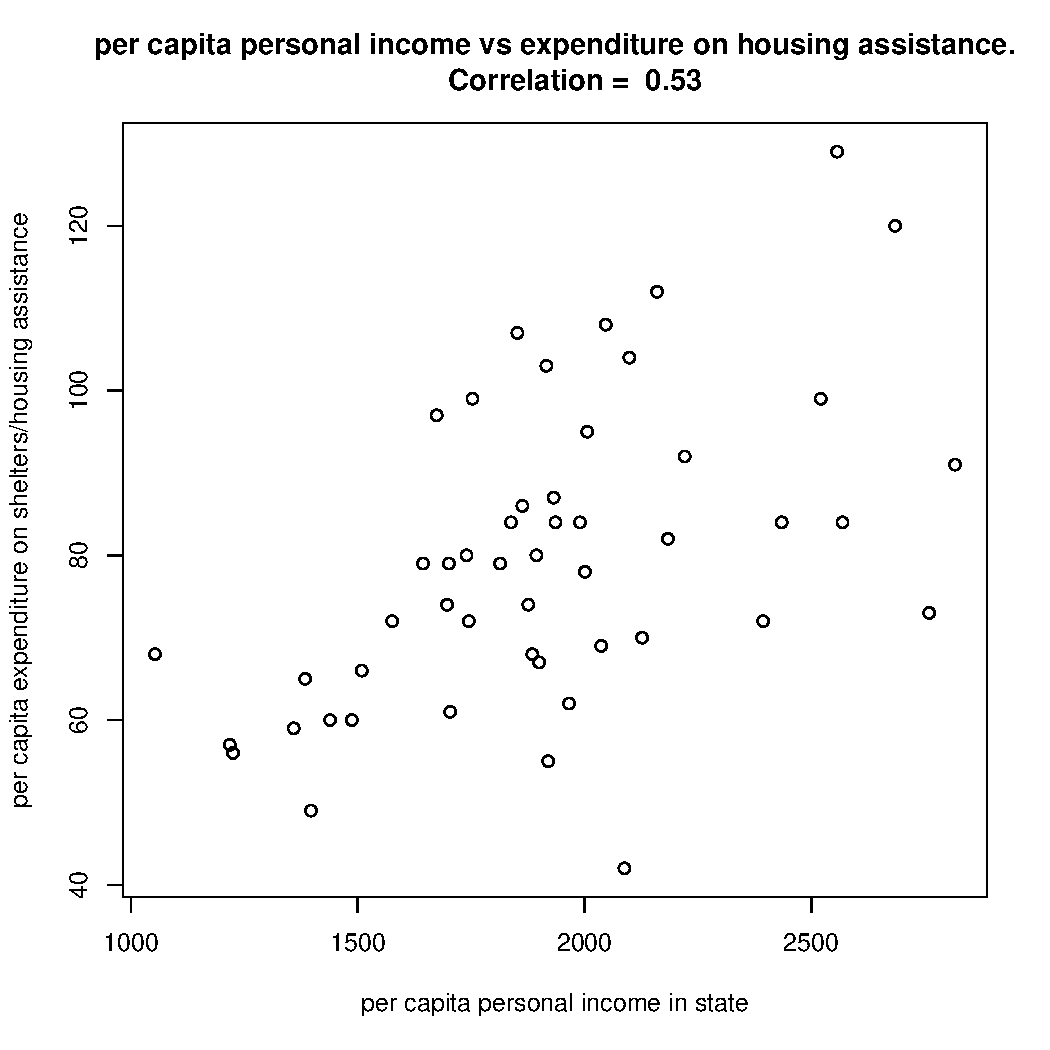
\includegraphics[width=10cm]{plot_Y_X1.pdf}  
\end{center}

\textcolor{blue}{
	\textbf{Interpretation of results:}\\
We can see that the variables are associated and the correlation value is also moderately high (0.53). This means, the per capita personal income has some relation with the per capita expenditure on housing assistance in state.
}

\pagebreak

\textcolor{blue}{
	\noindent \textbf{\texttt{R} script used for calculating the correlation values and plotting the relationship between Y and X2:}
}

\lstinputlisting[language=R, firstline=98, lastline=108]{PS01_answers_SK.R}  

\vspace{.25cm}

\textcolor{blue}{
	\noindent \textbf{The following graph shows the relationship between Y and X2:}
}
\begin{center}
	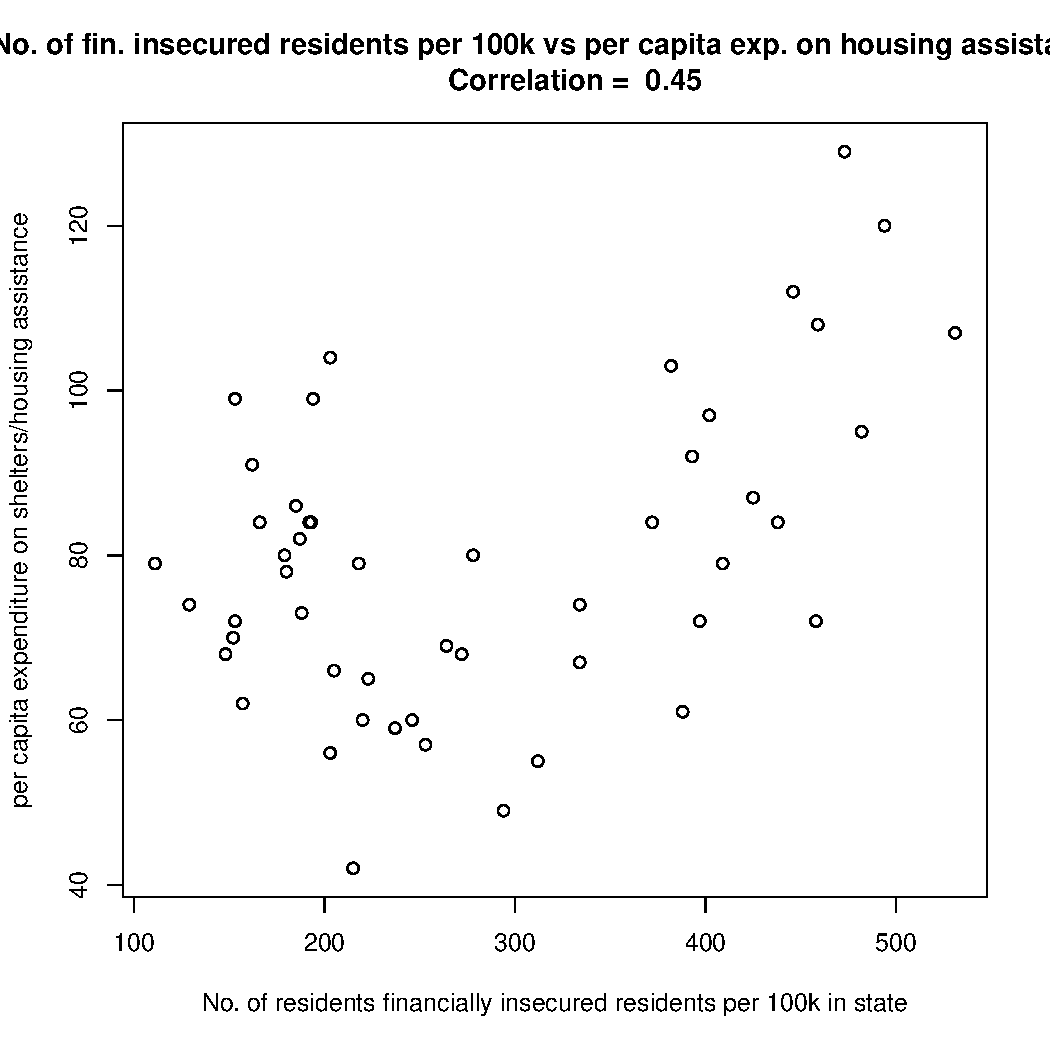
\includegraphics[width=10cm]{plot_Y_X2.pdf}  
\end{center}

\textcolor{blue}{
	\textbf{Interpretation of results:}\\
	We can see that the variables are mildly associated and the correlation value is also moderate (0.45). However, we also see a lot of dispersions in per capita expenditure on housing assistance with lower values of number of residents financially insecured per 100k in state. 
}

\pagebreak

\textcolor{blue}{
	\noindent \textbf{\texttt{R} script used for calculating the correlation values and plotting the relationship between Y and X3:}
}

\lstinputlisting[language=R, firstline=110, lastline=120]{PS01_answers_SK.R}  

\vspace{.25cm}

\textcolor{blue}{
	\noindent \textbf{The following graph shows the relationship between Y and X3:}
}
\begin{center}
	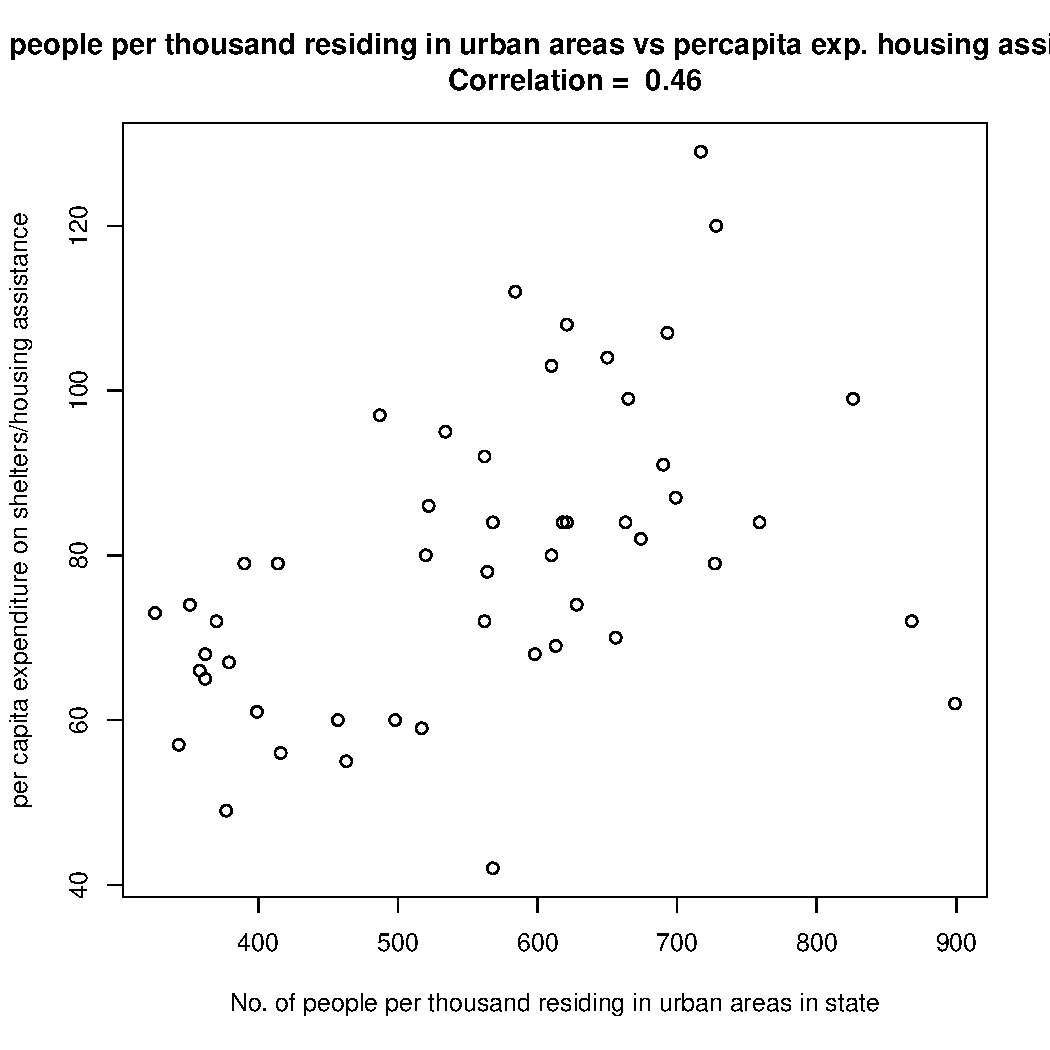
\includegraphics[width=10cm]{plot_Y_X3.pdf}  
\end{center}

\textcolor{blue}{
	\textbf{Interpretation of results:}\\
	We can see that the variables are mildly associated and the correlation value is also moderate (0.46). However, we see that there are some outliers in the data especially with higher values of number of people per thousand residing in urban areas in state.
}

\pagebreak

\textcolor{blue}{
	\noindent \textbf{\texttt{R} script used for calculating the correlation values and plotting the relationship between X1 and X2:}
}

\lstinputlisting[language=R, firstline=122, lastline=132]{PS01_answers_SK.R}  

\vspace{.25cm}

\textcolor{blue}{
	\noindent \textbf{The following graph shows the relationship between X1 and X2:}
}
\begin{center}
	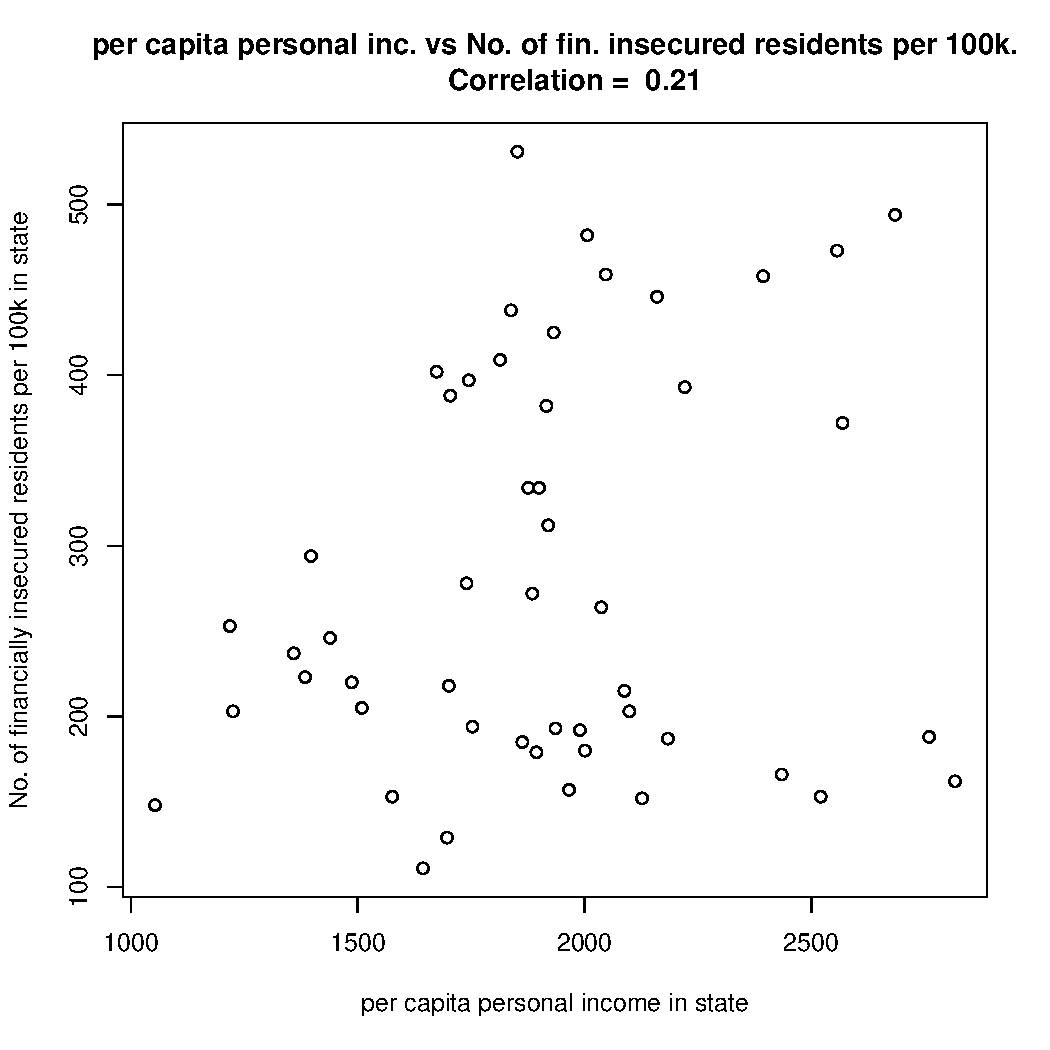
\includegraphics[width=10cm]{plot_X1_X2.pdf}  
\end{center}

\textcolor{blue}{
	\textbf{Interpretation of results:}\\
	We can see that the variables are not associated and the correlation value is also very low (0.21). This means, the per capita personal income has no relation with number of financially insecured residents per 100k in state.
}

\pagebreak

\textcolor{blue}{
	\noindent \textbf{\texttt{R} script used for calculating the correlation values and plotting the relationship between X1 and X3:}
}

\lstinputlisting[language=R, firstline=134, lastline=144]{PS01_answers_SK.R}  

\vspace{.25cm}

\textcolor{blue}{
	\noindent \textbf{The following graph shows the relationship between X1 and X3:}
}
\begin{center}
	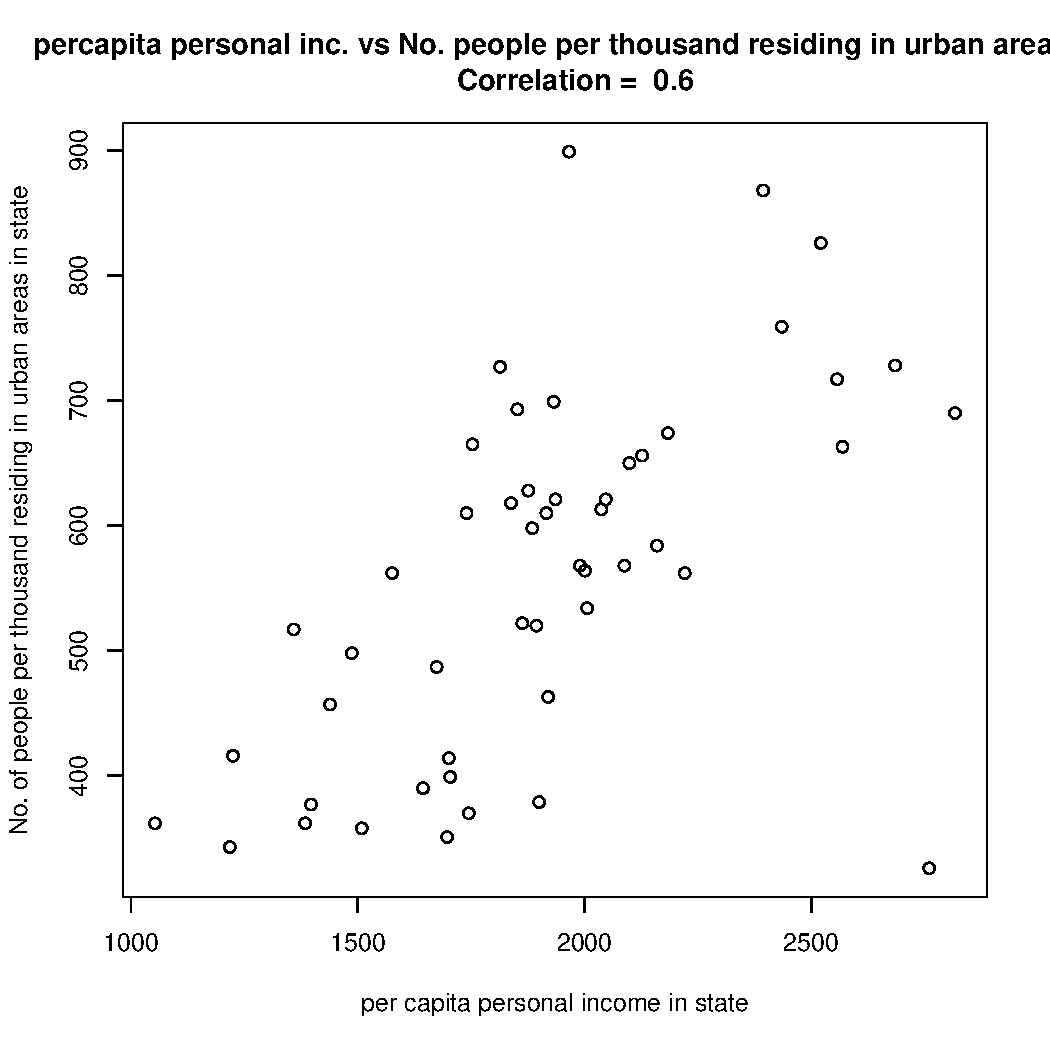
\includegraphics[width=10cm]{plot_X1_X3.pdf}  
\end{center}

\textcolor{blue}{
	\textbf{Interpretation of results:}\\
	We can see that the variables are associated and the correlation value is also moderately high (0.60). This means, the per capita personal income has some relation with number of people per thousand residing in urban areas in state.
}

\pagebreak

\textcolor{blue}{
	\noindent \textbf{\texttt{R} script used for calculating the correlation values and plotting the relationship between X2 and X3:}
}

\lstinputlisting[language=R, firstline=146, lastline=156]{PS01_answers_SK.R}  

\vspace{.25cm}

\textcolor{blue}{
	\noindent \textbf{The following graph shows the relationship between X2 and X3:}
}
\begin{center}
	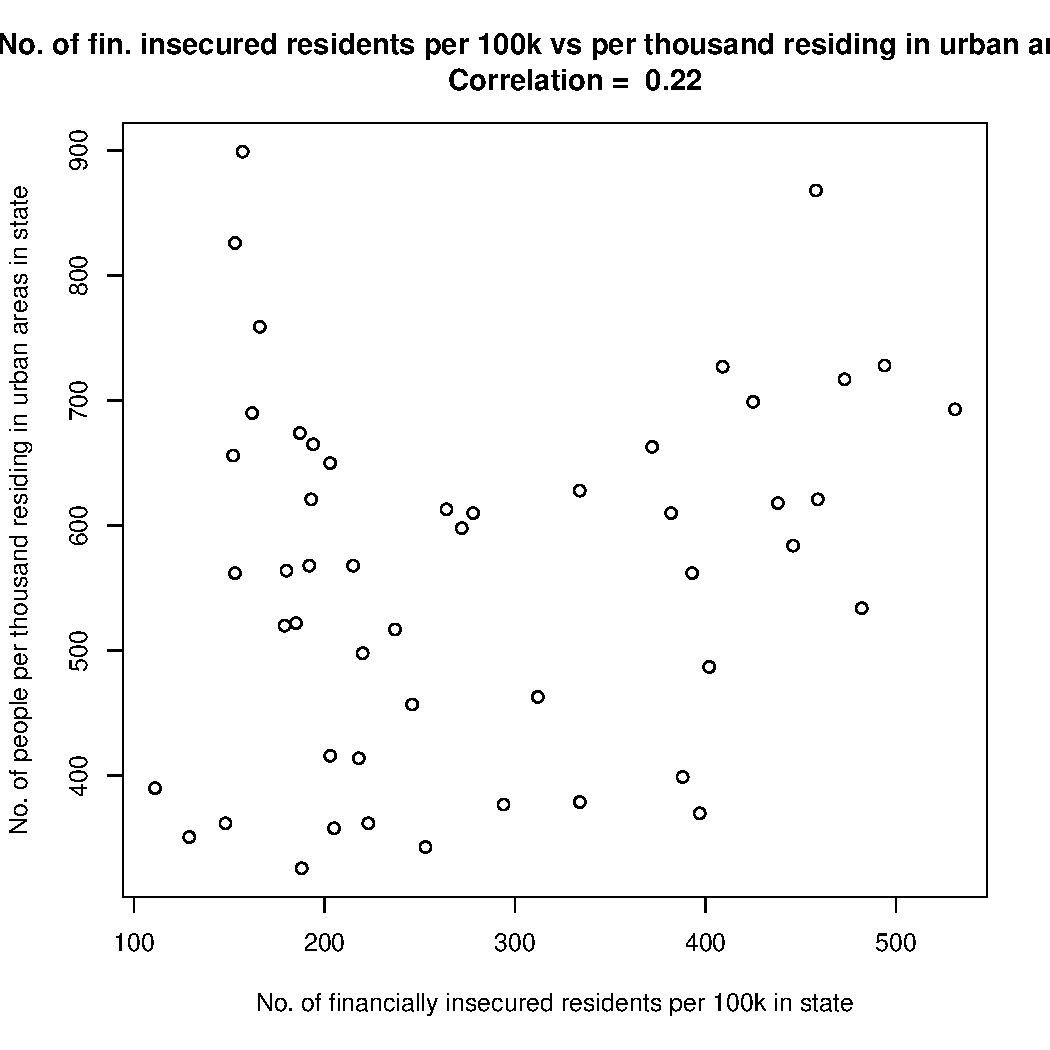
\includegraphics[width=10cm]{plot_X2_X3.pdf}  
\end{center}

\textcolor{blue}{
	\textbf{Interpretation of results:}\\
	We can see that the variables are not associated and the correlation value is also very low (0.22). This means, the number of financially insecured residents per 100k has no relation with number of people per thousand residing in urban areas in state.
}

\pagebreak

\item
Please plot the relationship between \emph{Y} and \emph{Region}? On average, which region has the highest per capita expenditure on housing assistance?
\vspace{.25cm}

\textcolor{blue}{
	\noindent \textbf{\texttt{R} script used for plotting the relationship between Y and Region:}
}

\lstinputlisting[language=R, firstline=160, lastline=170]{PS01_answers_SK.R}  

\textcolor{blue}{
	\noindent \textbf{The following graph shows the relationship between Y and Region:}
}
\begin{center}
	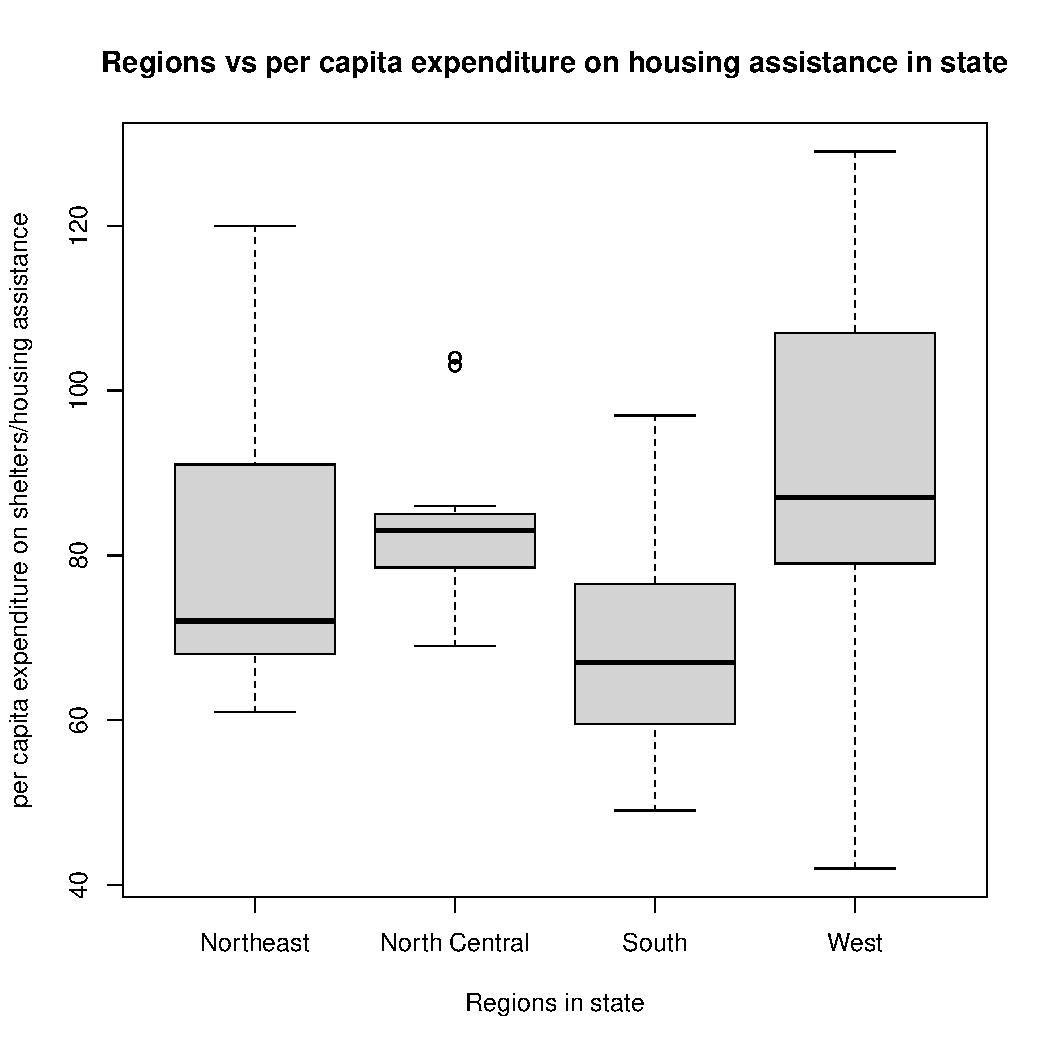
\includegraphics[width=10cm]{plot_Y_Region.pdf}  
\end{center}

\textcolor{blue}{
	\textbf{Interpretation of results:}\\
	From the above boxplot visually we see that the median for \textit{Region} 4 or \textit{West} is greater than other regions. We also calculated the mean (mentioned in the \texttt{R} script) and found that on average, \textit{Region} 4 (\textit{West}) has the highest per capita expenditure on housing assistance with 88.30769.
}

\pagebreak

\item
Please plot the relationship between \emph{Y} and \emph{X1}? Describe this graph and the relationship. Reproduce the above graph including one more variable \emph{Region} and display different regions with different types of symbols and colors.

\textcolor{blue}{
	\noindent \textbf{\texttt{R} script used for calculating the correlation values and plotting the relationship between Y and X1:}
}

\lstinputlisting[language=R, firstline=185, lastline=194]{PS01_answers_SK.R}  

\vspace{.25cm}

\textcolor{blue}{
	\noindent \textbf{The following graph shows the relationship between Y and X1:}
}
\begin{center}
	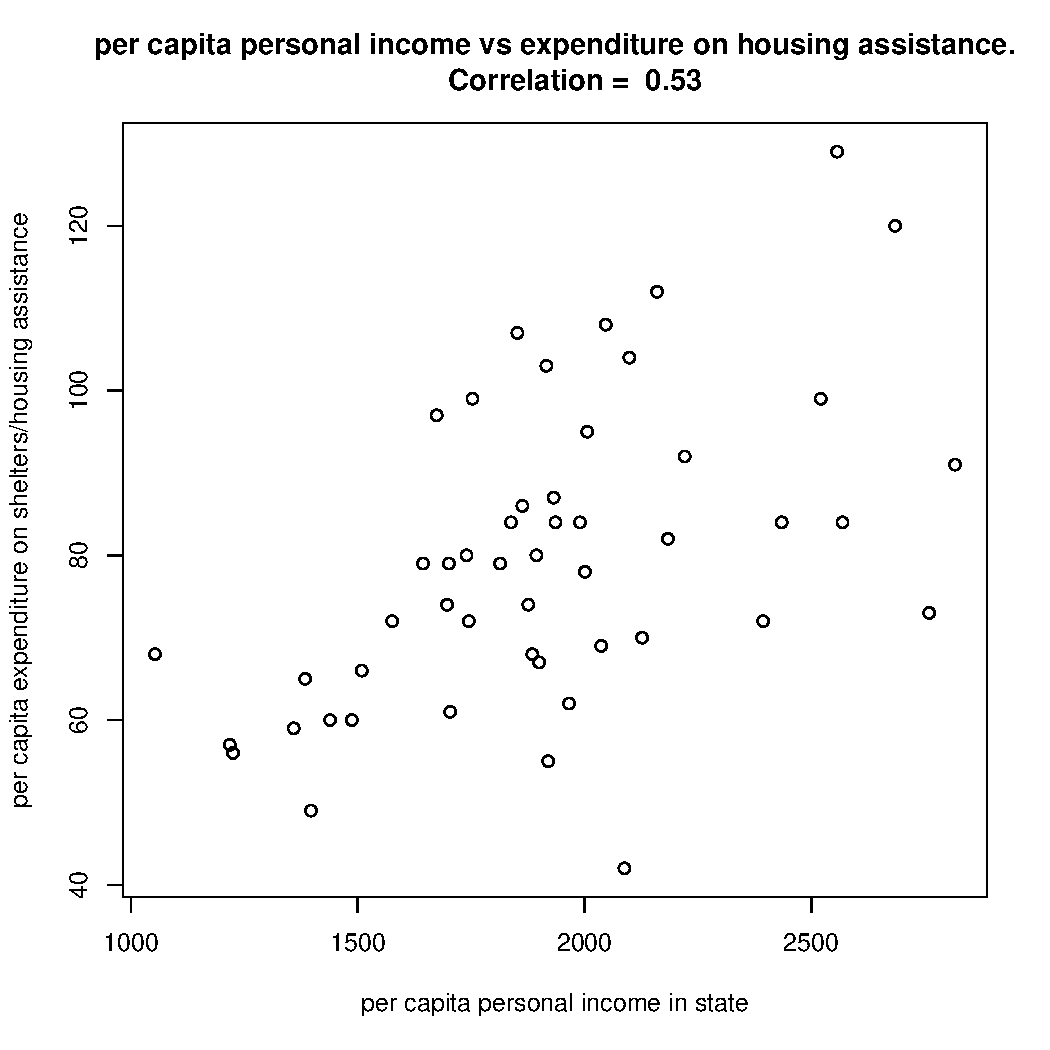
\includegraphics[width=10cm]{plot_Y_X1.pdf}  
\end{center}

\textcolor{blue}{
	\textbf{Interpretation of results:}\\
	As discussed in 2.1, we can see that the variables are associated and the correlation value is also moderately high (0.53). Indicating, the per capita personal income has some relation with the per capita expenditure on housing assistance in state.
}
\pagebreak

\textcolor{blue}{
	\textbf{Reproducing the graph including the \textit{Region} variable and displaying the regions with different types of symbols and colours.\\}
	\noindent \textbf{\\Following \texttt{R} script is used:}
}

\lstinputlisting[language=R, firstline=196, lastline=208]{PS01_answers_SK.R}  

\textcolor{blue}{
	\noindent \textbf{The following graph shows the relationship between Y and X1 alongwith the \textit{Region} variable:}
}
\begin{center}
	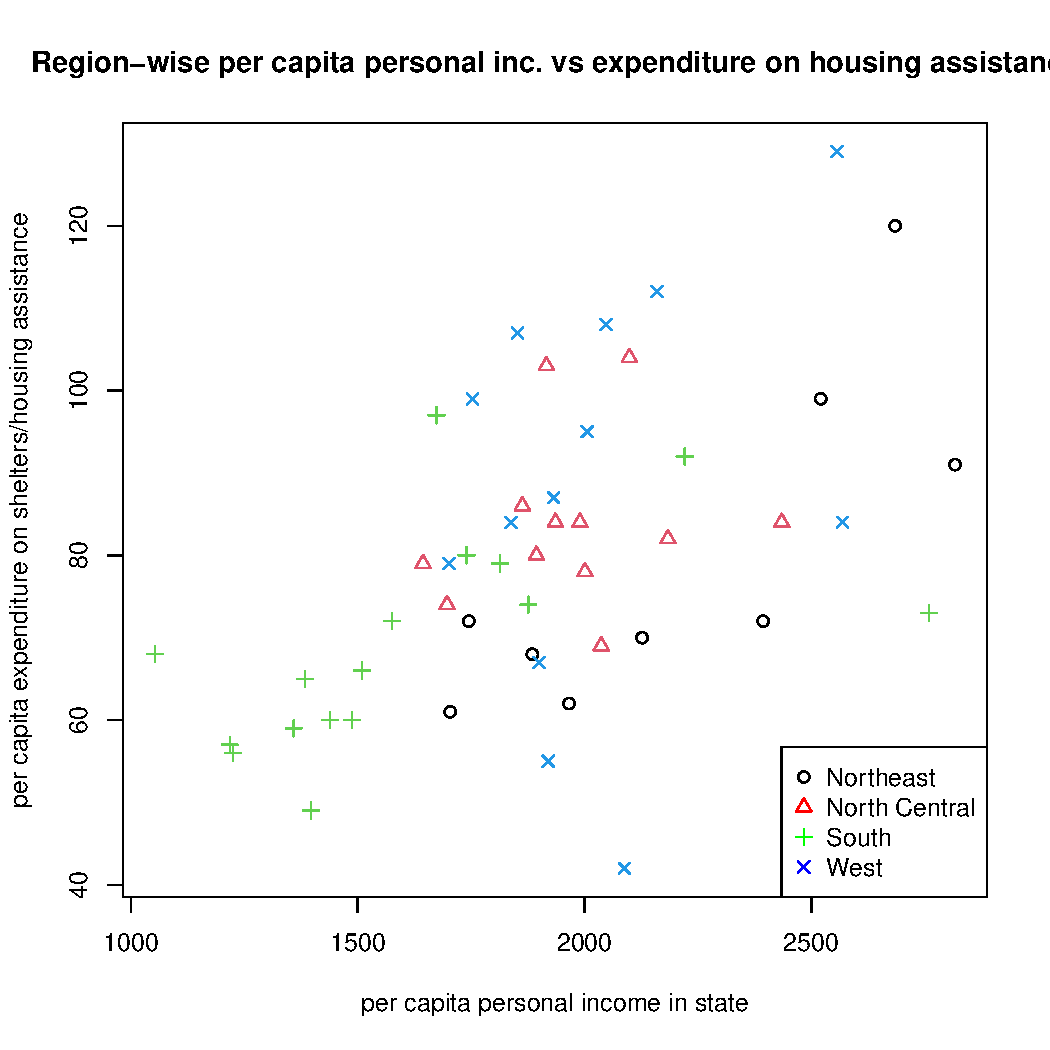
\includegraphics[width=11cm]{plot_Y_X1_new.pdf}  
\end{center}

\pagebreak

\textcolor{blue}{
	\textbf{Interpretation of results:}\\
\begin{itemize}
\item Firstly, as explained above, we can see the per capita personal income has some relation (correlation value = 0.53) with the per capita expenditure on housing assistance in state. In terms of region, we see \textit{Region} 4 or the \textit{West} region takes on an average greater value for per capita expenditure on housing assistance for any given value of per capita personal income in state.
\item \textit{Region} 2 or the \textit{North Central} region is mostly clustered around the middle of the graph with the least dispersion.
\item Furthermore, the \textit{Region} 1 or \textit{Northeast} and \textit{Region} 3 or \textit{South} region are widely dispersed with \textit{Region} 1 mostly taking higher values of per capita personal income compared to \textit{Region} 3 which takes mostly lower values of per capita personal income. Also, the mean per capita expenditure on housing assistance for \textit{Region} 1 is higher than \textit{Region} 3.
\end{itemize}
}

\end{itemize}
\vspace{2cm}
\begin{center}
\textcolor{blue}{\textbf{End of document}\\}
\end{center}
\vspace{10cm}
\textcolor{red}{Last edits made on: \today}

\end{document}
